\documentclass[a4paper]{article}

\usepackage[a4paper, top=2cm, bottom=2cm, left=2cm, right=2cm]{geometry}
\usepackage[T1, T2A]{fontenc}
\usepackage[fontsize=12pt]{fontsize}

\usepackage[english, russian]{babel}
\usepackage[utf8]{inputenc}

\usepackage{hyperref}
\usepackage{amsthm}
\usepackage{tabularx}
\usepackage{pgfplots}
\usepackage{graphicx}
\usepackage{float}
\usepackage{tikz}
\usepackage{gensymb}
\usepackage{indentfirst}
\usepackage{amssymb}

\hypersetup{pdfpagemode=FullScreen, colorlinks=true, linkcolor=black, urlcolor=cyan}

\newtheoremstyle{mainstyle}
{\topsep} % measure of space to leave above the theorem
{\topsep} % measure of space to leave below the theorem
{\normalfont} % name of font to use in the body of the theorem
{0pt} % measure of space to indent
{\large\bfseries} % name of head font
{\newline\null} % punctuation between head and body
{\parindent} % space after theorem head
{\thmname{#1}\thmnumber{ #2}\textnormal{\thmnote{ (#3)}}}

\newcommand{\definitionfont}[1]{\textit{#1}}

\theoremstyle{mainstyle}
\newtheorem*{definition}{Определение}
\newtheorem*{goal}{Цель}
\newtheorem*{remark}{Замечание}
\newtheorem*{criteria}{Критерий}
\begin{document}	
	\begin{titlepage}
	\centering
	{\LARGE \textsc{НОВОСИБИРСКИЙ ГОСУДАРСТВЕННЫЙ УНИВЕРСИТЕТ}\par}
	{\textsc{ФАКУЛЬТЕТ ИНФОРМАЦИОННЫХ ТЕХНОЛОГИЙ}\par}
	
	\vspace{3cm}
	
	{\huge\bfseries Основы теории управления\par}
	
	\vspace{1cm}
	
	{\Large\bfseries Задание 3. Анализ устойчивости регуляторов по критерию Найквиста\par}
	
	\vspace{10cm}
	
	\begin{flushright}
		{\large\textit{Выполнил}}
		
		Кондренко К.П., группа 21203
		
		\bigskip
		
		{\large\textit{Преподаватель}}
		
		Ломов А.А.
	\end{flushright}
	
	\vfill
	
	{\large \today\par}
\end{titlepage}

	
	\newpage
	
	\tableofcontents
	
	\newpage
	
	\section{Введение}
	\begin{goal}
		Исследование и анализ устойчивости регуляторов по критерию Найквиста.
	\end{goal}
	
	\begin{definition}
		\definitionfont{Годограф Найквиста} --- это функция
		\[v (iw) = W(iw),\]
		
		где $W(s)$ --- передаточная функция рассматриваемой системы.		
	\end{definition}
	
	\begin{criteria}[Найквиста при использовании ЛЧХ]
		Система устойчива тогда и только тогда, когда годограф Найквиста не охватывает точку $(-1; 0)$.
	\end{criteria}
\section{Постановка задачи}
	\begin{definition}
		\definitionfont{Запасом устойчивости по амплитуде} называется число
		\[K_a = 20 \log \frac{1}{a},\]
		
		где $a$ --- расстояние от годографа Найквиста до точки $(-1; 0)$.
	\end{definition}

	\begin{definition}
		\definitionfont{Запасом устойчивости по фазе} называется число $\Delta \varphi$, равняющееся углу $\llcorner -1;0;A \lrcorner$, где $A$ --- точка, лежащая на единичной окружности (с центром в нуле) и принадлежащая годографу Найквиста.
	\end{definition}

	\begin{remark}
		Достаточным считается запас устойчивости по фазе не менее 30-60 градусов, а по амплитуде не менее 6-12 дБ.
	\end{remark}

	\begin{remark}
		Требуется определить запас устойчивости по фазе и по амплитуде для систем автоматического управления с объектом управления из задания №1 при
		одном значении чистого запаздывания с ПИ и ПИД-регуляторами. Параметры ПИ и ПИД-регуляторов получены при выполнении задания №1 оптимальной
		настройкой по интегральному критерию качества.
	\end{remark}
\section{Схемы и результаты моделирования}
	\begin{figure}[H]
		\centering
		
\includegraphics[scale=0.4]{./images/7.png}
		\caption{Схема моделирования частотных характеристик с ПИ-регулятором} 
	\end{figure}
	
	\begin{figure}[H]
		\centering
		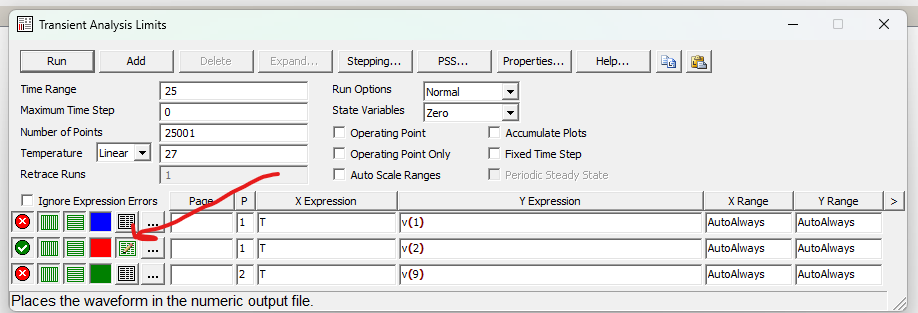
\includegraphics[scale=0.4]{./images/1.png}
		\caption{Схема моделирования частотных
			характеристик с ПИД-регулятором} 
	\end{figure}
	
	\begin{table}[H]
		\centering
		\begin{tabularx}{\textwidth}{
				| >{\arraybackslash}X
				| >{\arraybackslash}X
				| >{\arraybackslash}X
				| >{\arraybackslash}X
				|}
			\hline
			$\mathbf{a}$ & $\mathbf{K_a}$, dB & $\mathbf{\varphi}, \degree$ & $\mathbf{\Delta \varphi}, \degree$\\\hline
			0.602 & 4.406 & 245 & 65 \\\hline
		\end{tabularx}
		\caption{Результаты исследования запаса устойчивости с ПИ-регулятором}
	\end{table}
	
	\begin{table}[H]
		\centering
		\begin{tabularx}{\textwidth}{
				| >{\arraybackslash}X
				| >{\arraybackslash}X
				| >{\arraybackslash}X
				| >{\arraybackslash}X
				|}
			\hline
			$\mathbf{a}$ & $\mathbf{K_a}$, dB & $\mathbf{\varphi}, \degree$ & $\mathbf{\Delta \varphi}, \degree$\\\hline
			0.587 & 4.62 & 253 & 73 \\\hline
		\end{tabularx}
		\caption{Результаты исследования запаса устойчивости с ПИД-регулятором}
	\end{table}
\section{Выводы}
	Проведённый анализ показывает, что ПИ-регулятор для рассматриваемого объекта имеет меньший запас устойчивости (и по амплитуде, и по фазе) по сравнению с ПИД-регулятором для того же объекта.
\section{Приложения}
	\begin{figure}[H]
		\centering
		
\includegraphics[scale=0.35]{./images/3.png}
		
\includegraphics[scale=0.35]{./images/4.png}
		\caption{Определение запаса устойчивости по амплитуде для ПИД-регулятора} 
	\end{figure}
	
	\begin{figure}[H]
		\centering
		
\includegraphics[scale=0.35]{./images/5.png}
		
\includegraphics[scale=0.35]{./images/6.png}
		\caption{Определение запаса устойчивости по фазе для ПИД-регулятора} 
	\end{figure}
	
	\begin{figure}[H]
		\centering
		
\includegraphics[scale=0.35]{./images/9.png}
		
\includegraphics[scale=0.35]{./images/10.png}
		\caption{Определение запаса устойчивости по амплитуде для ПИ-регулятора} 
	\end{figure}
	
	\begin{figure}[H]
		\centering
		
\includegraphics[scale=0.35]{./images/11.png}
		
\includegraphics[scale=0.35]{./images/12.png}
		\caption{Определение запаса устойчивости по фазе для ПИ-регулятора} 
	\end{figure}
\end{document}
